\documentclass[12pt, a4paper]{article}
    
\usepackage{homework}
\usepackage{amsmath}				% For Math
\usepackage{fancyhdr}				% For fancy header/footer
\usepackage{graphicx}				% For including figure/image
\usepackage{cancel}					% To use the slash to cancel out stuff in work
\usepackage{multirow}

%%%%%%%%%%%%%%%%%%%%%%
% Set up fancy header/footer
\pagestyle{fancy}
\setlength{\headheight}{42pt}
\fancyhead[LO,L]{Name: Yu Ching Hei\\SID: 1155193237\\email: chyu2@cse.cuhk.edu.hk}
\fancyhead[CO,C]{}
\fancyhead[RO,R]{CENG3420 Computer Organization and Design\\Homework 3\\Date: \today}
\fancyfoot[LO,L]{}
\fancyfoot[CO,C]{}
\fancyfoot[RO,R]{Page \thepage}
\renewcommand{\headrulewidth}{0.4pt}
\renewcommand{\footrulewidth}{0.4pt}
%%%%%%%%%%%%%%%%%%%%%%

\begin{document}

\begin{q}{20}
    Consider two different implementations of the same instruction set architecture. The
instructions can be divided into three classes according to their CPI (classes A, B, and
C). P1 with a clock rate of 2.5 GHz and CPIs of 1, 2 and 3, and P2 with a clock rate of
2 GHz and CPIs of 2, 2 and 2. A program with an instruction count of 1 × 10$^7$ can be
divided into classes as follows: 20\% class A, 50\% class B, 30\% class C. 
\begin{enumerate}
    \item What is the average CPI for each implementation? (10\%)
    \item What is the CPU execution time of this program for each implementation? (10\%)
\end{enumerate}
\end{q}
\begin{ans}
\begin{enumerate}
    \item 
    \begin{itemize}
        \item P1: $$\sum_{i=1}^{3}\text{CPI}_i\times\text{IC}_i = 1\times0.2+2\times0.5+3\times0.3=2.1$$
        \item P2: $$\sum_{i=1}^{3}\text{CPI}_i\times\text{IC}_i = 2\times0.2+2\times0.5+2\times0.3=2$$
    \end{itemize}
    \item 
    \begin{itemize}
        \item P1: $$\text{CPU Time}=\frac{\text{IC}\times\text{CPI}}{\text{clock rate}}=\frac{1\times10^7\times2.1}{2.5\text{GHz}}=8.4\times10^{-3}$$
        \item P2: $$\text{CPU Time}=\frac{\text{IC}\times\text{CPI}}{\text{clock rate}}=\frac{1\times10^7\times2}{2\text{GHz}}=0.01$$
    \end{itemize}
\end{enumerate}
\end{ans}
\pagebreak

\begin{q}{15}
    Consider the following sequence of instructions, and assume that it is executed on a
five-stage pipelined datapath.
\begin{code}
    lw x12, 4(x11)
    lw x14, 4(x13)
    and x15, x12, x14
    sub x13, x11, x13
\end{code}
\begin{enumerate}
    \item If there is no forwarding or hazard detection, insert NOPs to ensure correct execution.
    You need to draw a pipeline diagram like we did in the lectures. (5\%)
    \item Does inserting NOPs change the clock cycle time? (5\%)
    \item Does inserting NOPs change the excute time of a program containing this block of
    code. (5\%)
\end{enumerate}
\end{q}
\begin{ans}
    \begin{enumerate}
        \item \text{ }\\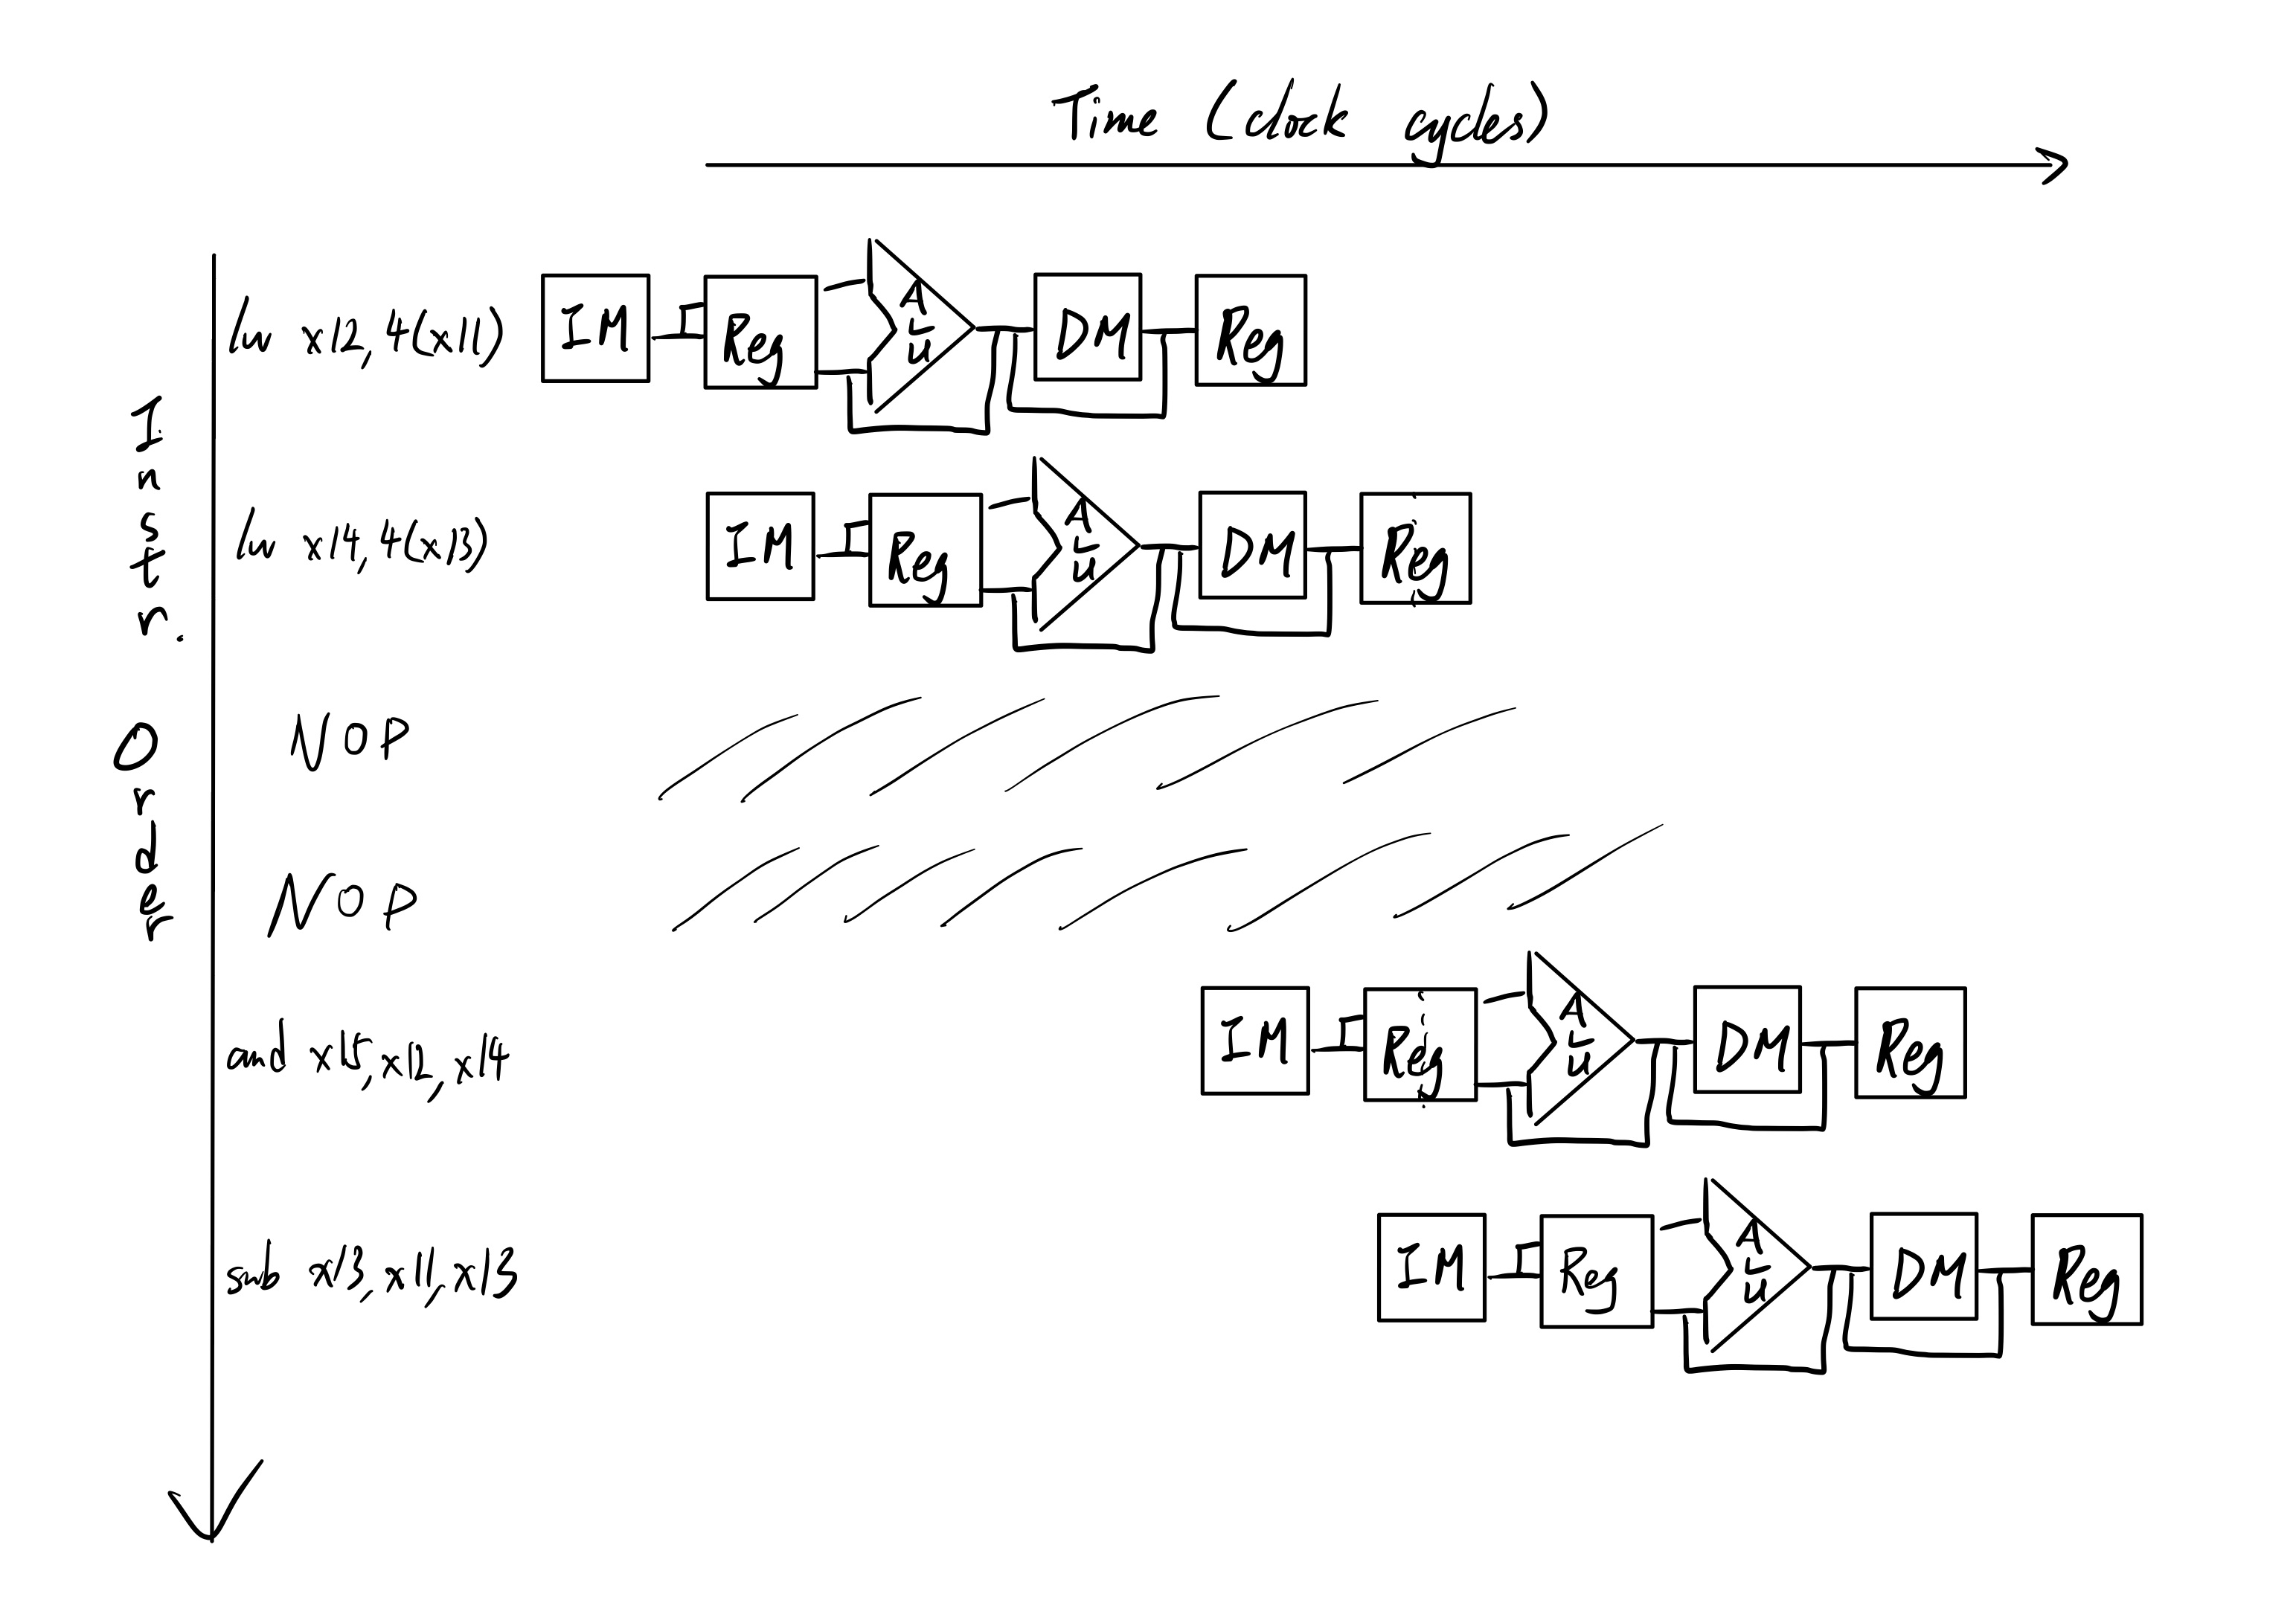
\includegraphics[width=1\linewidth]{../figs/q2.1-1.jpg}
        \item No, NOP will not affect clock cycle time
        \item Yes, since the program containing this block of code will require more clock cycles to finish. 
    \end{enumerate}
\end{ans}
\pagebreak

\begin{q}{25}
    Problems in this exercise refer to the following sequence of instructions, and suppose the
instructions are executed on a five-stage pipelined datapath.
\begin{code}
    or x4, x1, x3
    add x12, x4, x5
    sub x13, x6, x4
\end{code}
\begin{enumerate}
    \item List the data dependencies of the three instructions. (5\%)
    \item If there is no forwarding or hazard detection, how many NOPs are needed to ensure correct execution. You need to draw a pipeline diagram as we did in the lectures. (10\%)
    \item If hazard detection and forwarding are allowed, draw a pipeline diagram \textbf{only with forwarding} to ensure correct execution. In the diagram, the forwarding need to be specified by an arrow. (10\%)
\end{enumerate}
\end{q}
\begin{ans}
    \begin{enumerate}
        \item Write After Read(WAR)
        \item 2 NOPs are required \\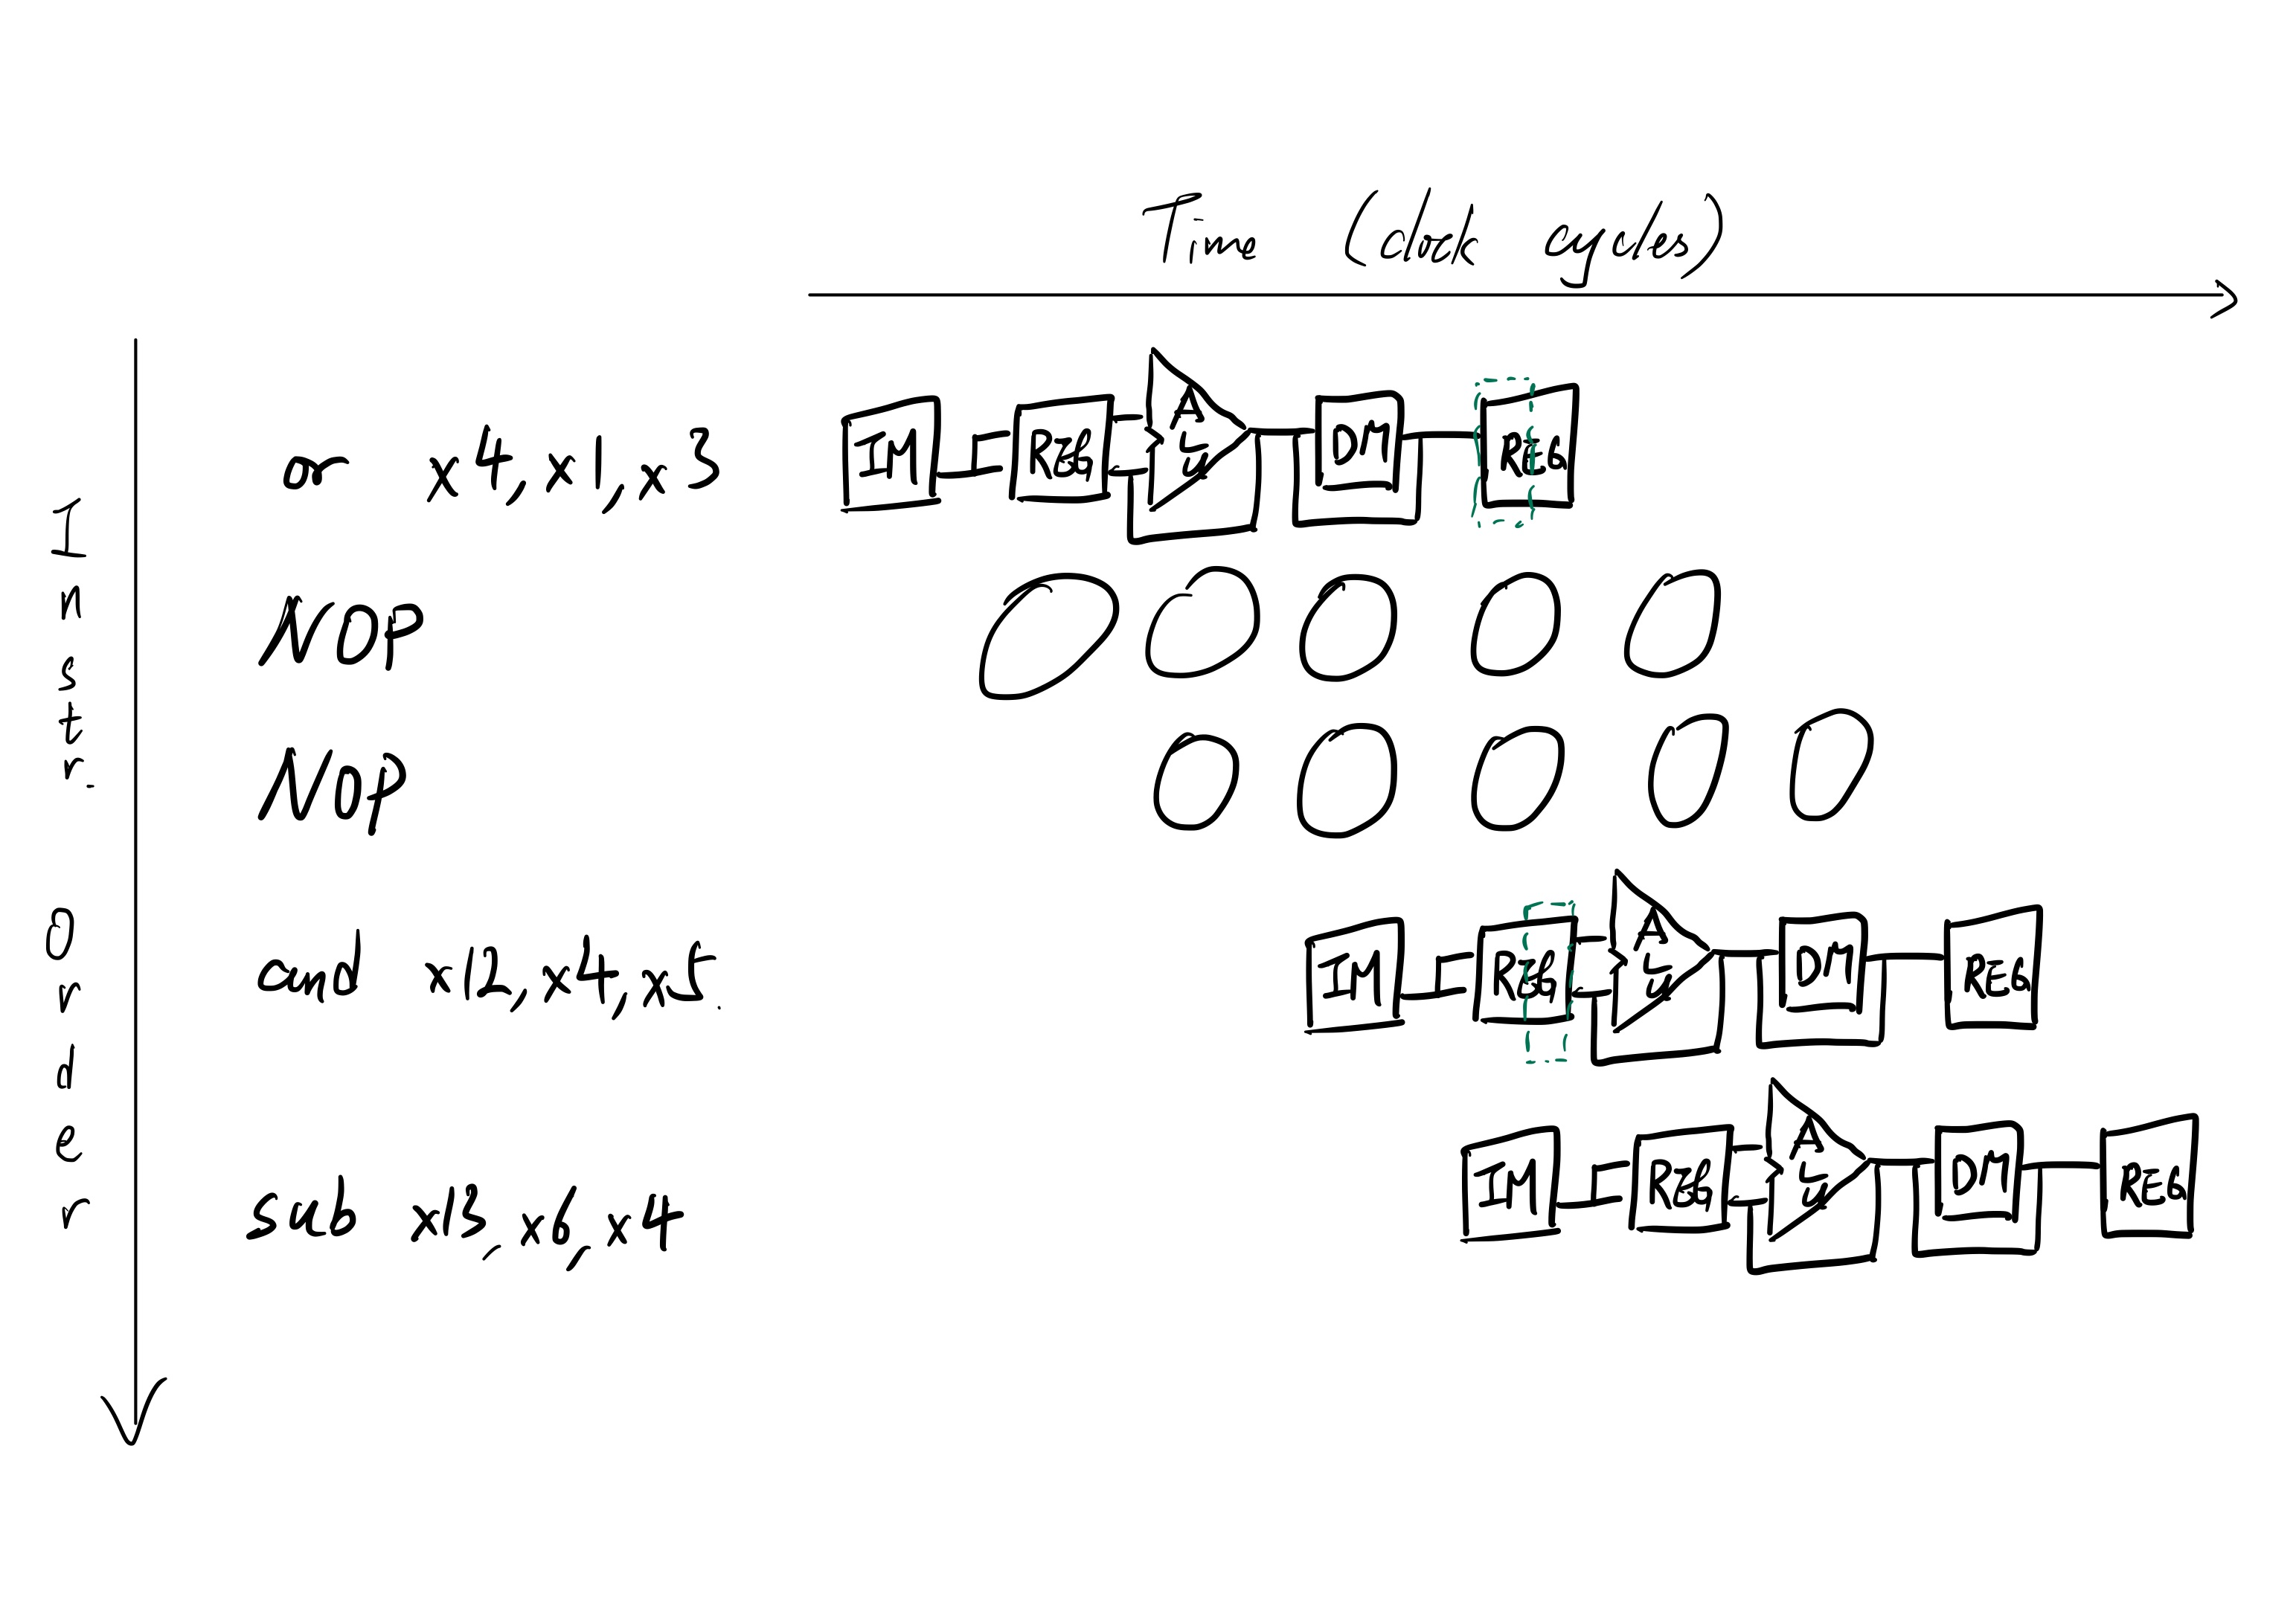
\includegraphics[width=.6\linewidth]{../figs/q3.2-2.jpg}
        \item \text{ }\\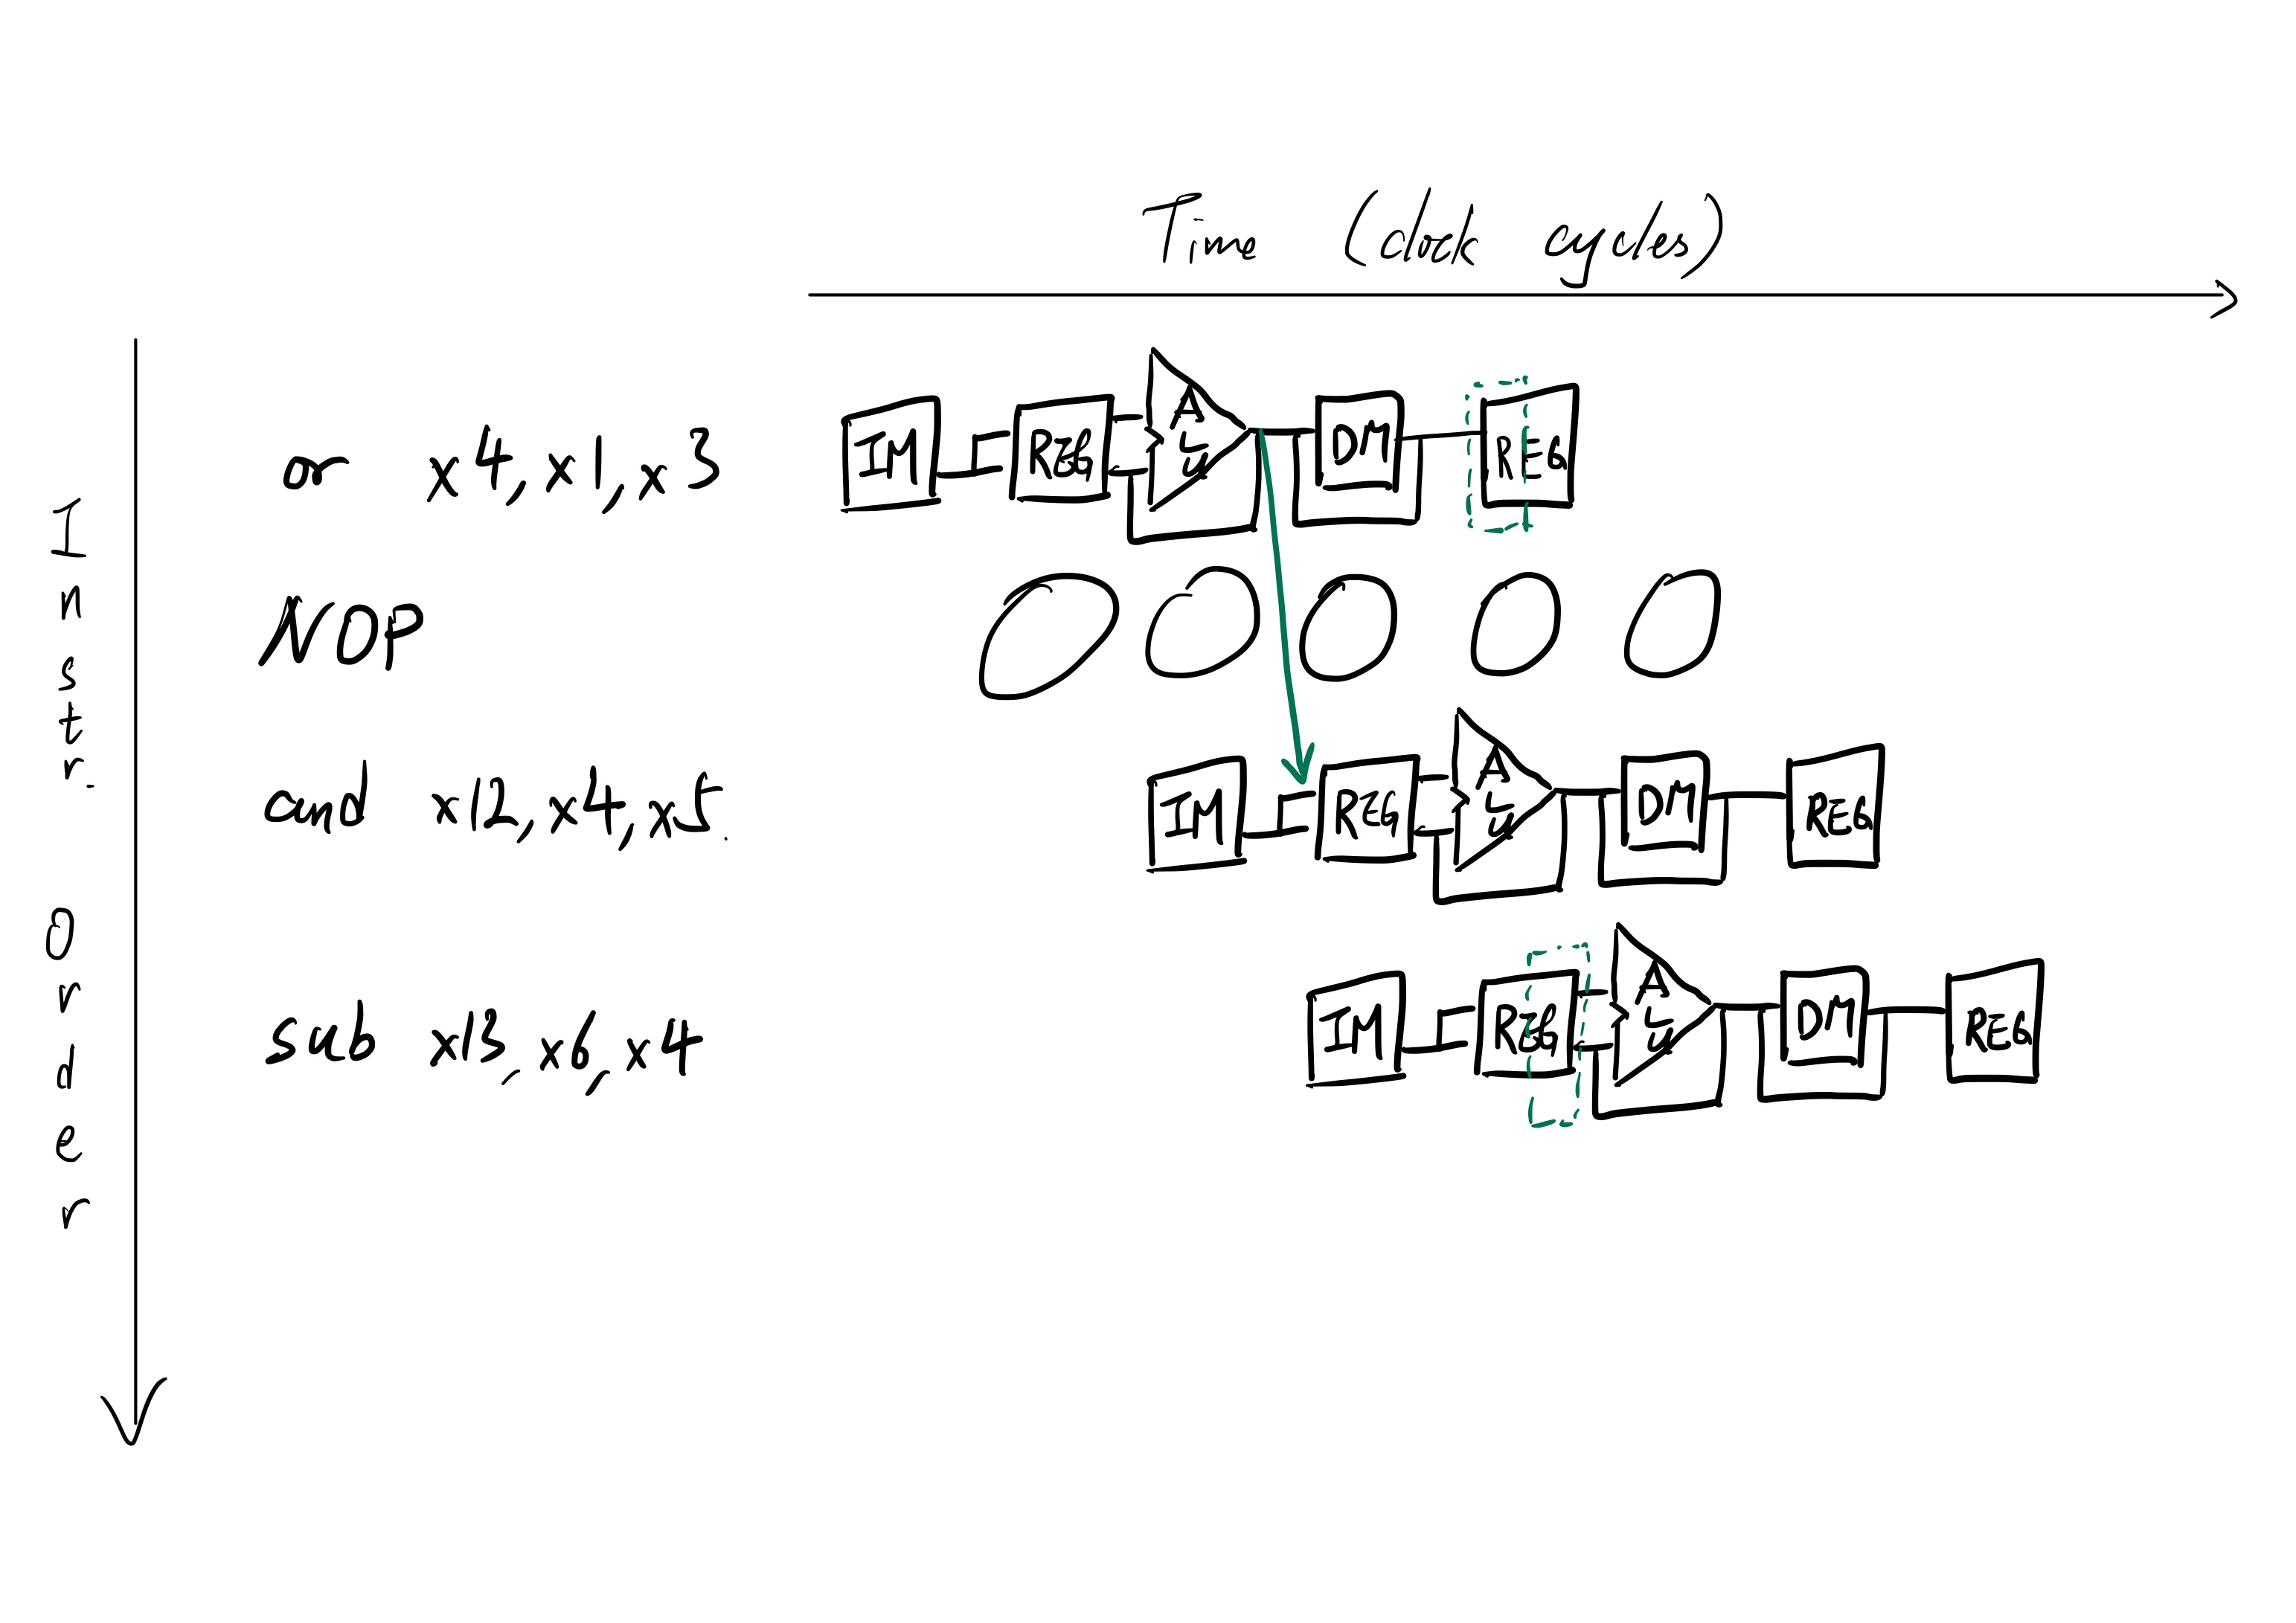
\includegraphics[width=.6\linewidth]{../figs/q3.3-3.jpg}
    \end{enumerate}
\end{ans}
\pagebreak

\begin{q}{20}
    This exercise examines the accuracy of various branch predictors for the following repeating pattern (e.g., in a loop) of branch outcomes: T, NT, NT, T, T. (T means ’Taken’ and NT means ’Not taken’)
    \begin{enumerate}
        \item What is the accuracy of always-taken and always-not-taken predictors for this sequence of branch outcomes? (5\%)
        \item What is the accuracy of a 2-bit predictor if this pattern is repeated forever? You should give your explanations rather than just an answer. The table below is recommended. The following figure shows the finite-state machine for a 2-bit prediction scheme. Here we assume this predictor starts from ”State 0”. (15\%)
    \end{enumerate}
\end{q}
\begin{ans}
    \begin{enumerate}
        \item 
        \begin{itemize}
            \item always-taken: 60\%
            \item always-not-taken: 40\%
        \end{itemize}
        \item 
        \begin{tabular}{|c|c|c|c|c|}
            \hline
             & Iteration1 & Iteration2 & Iteration3 & ...\\
            \hline
            Actual & T NT NT T T & T NT NT T T & T NT NT T T&...\\
            \hline
            Predictor State &0,1,0,0,1&2,3,2,1,2&3,3,2,1,2&3,3,2,1,2\\
            \hline
            Prediction & N,N,N,N,N & T,T,T,N,T & T,T,T,N,T & T,T,T,N,T \\
            \hline
            True or False & F,T,T,F,F & T,F,F,F,T & T,F,F,F,T & T,F,F,F,T\\
            \hline
        \end{tabular}
        \\$\therefore$ Accuracy= $2\div5$ = 40\%
    \end{enumerate}
\end{ans}
\pagebreak

\begin{q}{20}
    Assume a program requires the execution of 50 × 10$^6$ FP instructions, 110 × 10$^6$ INT instructions, 80 × 10$^6$ L/S instructions, and 16 × 10$^6$ branch instructions. The CPI for each type of instruction is 1, 1, 4, and 2, respectively. Assume that the processor has a 2 GHz clock rate. 
    \begin{enumerate}
        \item By how much must we reduce the CPI of L/S instructions if we want the program to run two times faster? (10\%)
        \item By how much is the execution time of the program improved if the CPI of INT and FP instructions is reduced by 40\% and the CPI of L/S and Branch is reduced by 30\%? (10\%)
    \end{enumerate}
\end{q}
\begin{ans}
    \begin{enumerate}
        \item 
        \text{Let k be the number of CPI to be reduced, t be the execution time}
        $$\frac{1t}{3t} = \frac{\frac{25}{128} + \frac{55}{128} + (4-k)\frac{5}{16} + 2\frac{1}{16}}{\frac{25}{128} + \frac{55}{128} + 4\frac{5}{16} + 2\frac{1}{16}}$$
        $$\frac{1t}{3t} = \frac{192+(4-k)80}{512}$$
        $$k = 2$$
        \item $$\frac{0.6*110 + 0.7*4*80 + 50 + 16*2}{110 + 4*80 + 50+16*2} = 72.6\%$$
    \end{enumerate}
\end{ans}
\end{document}
